\documentclass[12pt]{ximera}

\usepackage{nopageno}
\usepackage{amsmath}
\usepackage{graphicx}
\usepackage{geometry}
\geometry{top=1in,bottom=1in,right=0.75in,left=0.75in}
\usetikzlibrary{patterns}

\usepackage{fancyhdr}
\usepackage{lastpage}
 
\pagestyle{fancy}
\fancyhf{}
\rhead{\textsf{Form C}}
\lhead{\textsf{Calculus Knowledge Assessment v3}}
\rfoot{\textsf{Page \thepage\ of \pageref{LastPage}}}


\usepackage{multicol}
\setlength{\columnsep}{2cm}

\usepackage{enumitem}

\setitemize{noitemsep,topsep=0pt,parsep=0pt,partopsep=0pt}

\renewenvironment{multipleChoice}
{\begin{trivlist}\item[\hskip\labelsep\small\bfseries Choose the best answer:]
\hfil\begin{enumerate}\begin{multicols}{2}}
 {\end{multicols}\end{enumerate}\end{trivlist}}

\def\image{\begin{center}}
\def\endimage{\end{center}}

%\renewcommand{\choice}[2][]{\item \begin{minipage}[t]{2in}#2\end{minipage}\ifthenelse{\boolean{#1}}{\ifhandout \else \quad\checkmark\fi}{}}
\renewcommand{\choice}[2][]{\item \begin{minipage}[t]{2in}#2\end{minipage}\ifthenelse{\boolean{#1}}{\ifhandout \else  \fi}{}}


\begin{document}
\vspace{6ex}

\begin{minipage}{\textwidth}
\begin{problem}

  Consider the following graph of a function, $f$, as seen through this
  window frame.  What can we say about $f(1)$?
  \begin{image}
    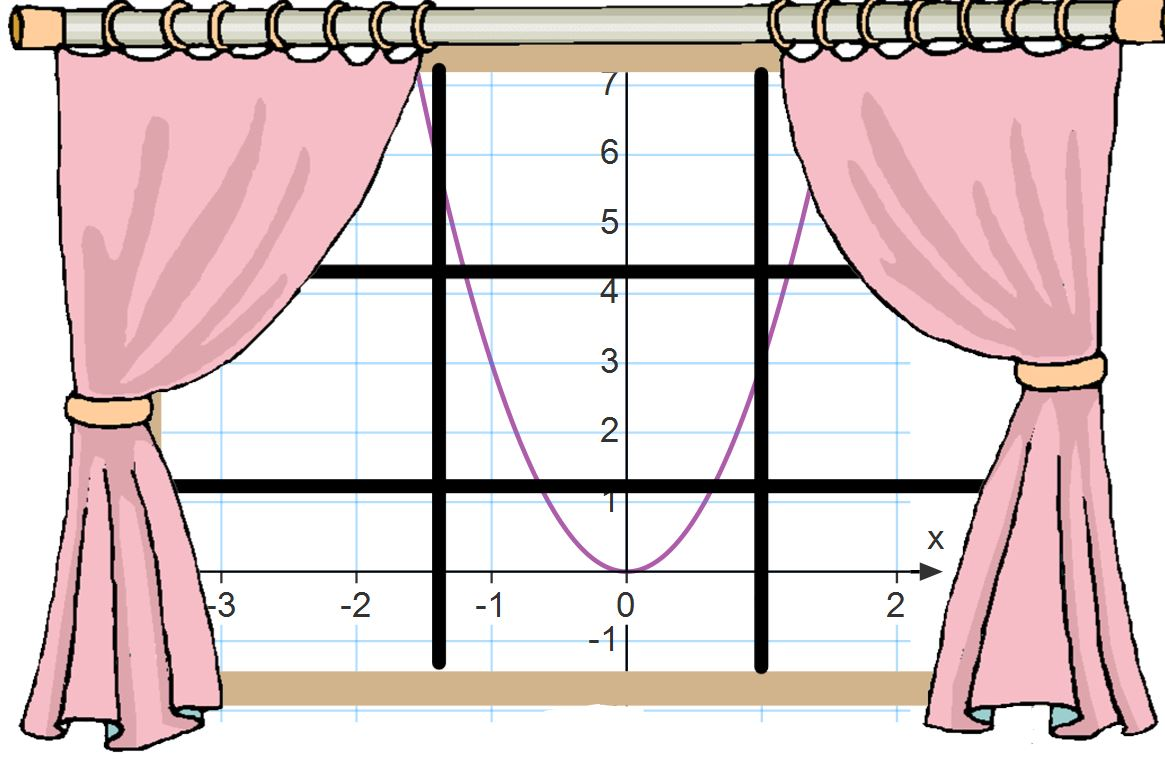
\includegraphics[scale= 0.25]{window}\\
  \end{image}
  \begin{multipleChoice}
    \choice{$f(1)=3$.}
    \choice{$f(1)$ is defined but we do not know it's value.}
    \choice{$f(1)$ is not defined.}
    \choice[correct]{We don't know anything about $f(1)$.}
  \end{multipleChoice}
\end{problem}
\end{minipage}

\vspace{6ex}

\begin{minipage}{\textwidth}
\begin{problem}
  %\recommendation{Elizabeth}
  % I fixed this to mention "at the origin"
  Suppose you are driving a car and you accelerate from a stopped
  position (at the origin) to 60 mph with a constant acceleration.
  Which graph below best resembles your position as a function of time
  over this time interval?
 
  \begin{multipleChoice}
    % increasing, concave up
    \choice[correct]{\begin{tikzpicture}[scale=0.33]\begin{axis}[clip=false,domain=0:1,ymin=-0.1,ymax=1.1,xmin=-0.1,xmax=1.1,xtick=\empty,ytick=\empty,axis lines=center,axis on top] \addplot [very thick, smooth] {x^2};\end{axis}\end{tikzpicture}}
    % increasing, concave down
    \choice{\begin{tikzpicture}[scale=0.33]\begin{axis}[clip=false,domain=0:1,ymin=-0.1,ymax=1.1,xmin=-0.1,xmax=1.1,xtick=\empty,ytick=\empty,axis lines=center,axis on top] \addplot [very thick, smooth,domain=0:1] ({x^2},{x});\end{axis}\end{tikzpicture}}
    % decreasing, concave down
    \choice{\begin{tikzpicture}[scale=0.33]\begin{axis}[clip=false,domain=0:1,ymin=-0.1,ymax=1.1,xmin=-0.1,xmax=1.1,xtick=\empty,ytick=\empty,axis lines=center,axis on top] \addplot [very thick, smooth,domain=0:1] ({x},{1-x^2});\end{axis}\end{tikzpicture}}
    % decreasing, concave up
    \choice{\begin{tikzpicture}[scale=0.33]\begin{axis}[clip=false,domain=0:1,ymin=-0.1,ymax=1.1,xmin=-0.1,xmax=1.1,xtick=\empty,ytick=\empty,axis lines=center,axis on top] \addplot [very thick, smooth,domain=0:1] ({x^2},{1-x});\end{axis}\end{tikzpicture}}
  \end{multipleChoice}
\end{problem}
\end{minipage}

\vspace{6ex}

\begin{minipage}{\textwidth}
\begin{problem}

  The graph of the position of an object with respect to time is given
  by a straight line with a positive slope.  What can we say about the
  acceleration of the object?
  \begin{multipleChoice}
    \choice{It is positive.}
    \choice{It is negative.}
    \choice[correct]{It is zero.}
    \choice{The acceleration changes from negative to positive.}
    \choice{We cannot say anything about the sign of the acceleration.}
  \end{multipleChoice}
\end{problem}
\end{minipage}

\vspace{6ex}

\begin{minipage}{\textwidth}
\begin{problem}

  Four numbers are shown below.
  \begin{image}
    \begin{tikzpicture}[x=0.19\textwidth]
      \draw[-{>[scale=1.75]}] (-0.05\textwidth,0) -- (0.8\textwidth,0);
      \foreach \x in {0,...,4} {%
        \draw (\x,-.1) -- (\x,.1);
        \node[anchor=north,yshift=-2pt] at (\x,0) {$\x$};
      }
      \draw (3.141592654,-.1) -- (3.141592654,.1);
      \node[anchor=north,yshift=-2pt] at (3.141592654,0) {$\pi$};
      \draw (0.25,0) node [circle,fill,inner sep=1pt,label=above:$x$](e){};
      \draw (0.65,0) node [circle,fill,inner sep=1pt,label=above:$y$](e){};
      \draw (3.3,0) node [circle,fill,inner sep=1pt,label=above:$z$](e){};
      \draw (3.8,0) node [circle,fill,inner sep=1pt,label=above:$w$](e){};
    \end{tikzpicture}
  \end{image}
  Let $f(x) = \sin x$.  What is true about $f(x)$, $f(y)$, $f(z)$, and $f(w)$?
  \begin{multipleChoice}
    \choice{$f(x) > f(y) > f(z) > f(w)$.}
    \choice{$f(x) > f(y) > f(w) > f(z)$.}
    \choice[correct]{$f(y) > f(x) > f(z) > f(w)$.}
    \choice{$f(y) > f(x) > f(w) > f(z)$.}
  \end{multipleChoice}
\end{problem}
\end{minipage}

\vspace{6ex}

\begin{minipage}{\textwidth}
\begin{problem} 

  Pick two numbers positve real numbers $a$ and $b$ so that
  $a \approx b$.  Pick a very large integer $N$.  What can you say
  about $a^N$ and $b^N$?
  \begin{multipleChoice}
    \choice{$a^N$ and $b^N$ must both be large because $N$ is large.}
    \choice{$a^N$ and $b^N$ must both be small because $|a-b|^N$ is small.}
    \choice{$a^N$ must be very close to $b^N$ because $a \approx b$.}
    \choice[correct]{$a^N$ might not be very close to $b^N$ even though $a \approx b$.}
  \end{multipleChoice}
\end{problem}
\end{minipage}

\vspace{6ex}

\begin{minipage}{\textwidth}
\begin{problem}
  
  Suppose $x$ is a number near one thousand, and $y$ is a number near $10^{10}$.  Which number below is nearest $x + y$?
  \begin{multipleChoice}
    \choice{$1000$}
    \choice[correct]{$10^{10}$}
    \choice{$10^{100}$}
    \choice{$10^{1000}$}
    \choice{$10^{1010}$}
  \end{multipleChoice}
\end{problem}
\end{minipage}

\vspace{6ex}

\begin{minipage}{\textwidth}
\begin{problem}

  Suppose whenever $x$ is very large, $f(x)$ is close to 1.  What is true about $f$?
  \begin{multipleChoice}
    \choice{The graph of $f$ does not cross the line $y = 1$.}
    \choice{The graph of $f$ does not cross the line $x = 1$.}
    \choice{Whenever $x$ is close to zero, $f(1/x)$ is close to 1.}
    \choice[correct]{Whenever $x$ is very large, $f(x^2)$ is close to 1.}
  \end{multipleChoice}
\end{problem}
\end{minipage}

\vspace{6ex}

\begin{minipage}{\textwidth}
\begin{problem}

  Suppose $f$ is an increasing function and $f(x) + g(x)$ is a constant.  How does $g$ depend on $x$?
  \begin{multipleChoice}
    \choice{$g$ must be increasing.}
    \choice{$g$ could be constant.}
    \choice[correct]{$g$ must be decreasing.}
    \choice{None of the above.}
  \end{multipleChoice}
\end{problem}
\end{minipage}

\vspace{6ex}

\begin{minipage}{\textwidth}
\begin{problem}

  Suppose $f$ and $g$ are increasing functions with domain consisting of all real numbers.  What can be said about the function $h(x) = f(g(x))$?
  \begin{multipleChoice}
    \choice{It is a decreasing function.}
    \choice{It is a constant function.}
    \choice[correct]{It is an increasing function.}
    \choice{It depends on exactly which functions $f$ and $g$ are being considered.}
  \end{multipleChoice}
\end{problem}
\end{minipage}

\vspace{6ex}

\begin{minipage}{\textwidth}
\begin{problem}

  Suppose $x$ is a positive number close to zero, and $y$ is a very large number.  What can be said about $y/x$?
  \begin{multipleChoice}
    \choice[correct]{It is very large.}
    \choice{It is close to zero.}
    \choice{It is very negative.}
    \choice{It could be very positive or very negative.}
  \end{multipleChoice}
\end{problem}
\end{minipage}

\vspace{6ex}

\begin{minipage}{\textwidth}
\begin{problem}
  Suppose $a$ and $b$ and $A$ and $B$ are very large, positive numbers, and suppose $A > a$ and $B < b$.  How does $A/B$ compare to $a/b$?
  \begin{multipleChoice}
    \choice[correct]{$A/B$ is bigger than $a/b$}
    \choice{$A/B$ is equal to $a/b$}
    \choice{$A/B$ is smaller than $a/b$}
    \choice{It could be that $A/B$ or $a/b$ is larger}
  \end{multipleChoice}
\end{problem}
\end{minipage}

\vspace{6ex}

\begin{minipage}{\textwidth}
\begin{problem}
  Suppose a polynomial $f$ achieves a global minimum, and besides that
  one point has no other local or global extrema.  What must be true
  of $f$?
  \begin{multipleChoice}
    \choice{$f'$ is a constant function}
    \choice{$f''$ is a constant function but it could be either negative or positive}
    \choice{$f''$ is a constant function and must be positive}
    \choice[correct]{None of these statements are true.}
  \end{multipleChoice}
\end{problem}
\end{minipage}

\vspace{6ex}

\begin{minipage}{\textwidth}
\begin{problem}
  Two pairs of numbers are shown below.
  \begin{image}
    \begin{tikzpicture}[x=0.19\textwidth]
      \draw[-{>[scale=1.75]}] (-0.05\textwidth,0) -- (0.8\textwidth,0);
      \foreach \x in {0,...,4} {%
        \draw (\x,-.1) -- (\x,.1);
        \node[anchor=north,yshift=-2pt] at (\x,0) {$\x$};
      }
      \draw (0.25,0) node [circle,fill,inner sep=1pt,label=above:$s$](e){};
      \draw (1.25,0) node [circle,fill,inner sep=1pt,label=above:$s+h$](e){};
      \draw (2.75,0) node [circle,fill,inner sep=1pt,label=above:$t$](e){};
      \draw (3.75,0) node [circle,fill,inner sep=1pt,label=above:$t+h$](e){};
    \end{tikzpicture}
  \end{image}
  Let $f(x) = -1/x$.  How does $f(s+h)-f(s)$ compare with $f(t+h) - f(t)$?
  \begin{multipleChoice}
    \choice{$f(s+h) - f(s) < f(t+h) - f(t)$}
    \choice{$f(s+h) - f(s) = f(t+h) - f(t)$}
    \choice[correct]{$f(s+h) - f(s) > f(t+h) - f(t)$}
  \end{multipleChoice}
\end{problem}
\end{minipage}

\vspace{6ex}

\begin{minipage}{\textwidth}
\begin{problem}
  Suppose $x, y, z$ are positive quantities which are depend on time
  $t$.  If $xyz = 1$ and $x$ is increasing, what must be true of $y$ and $z$?
  \begin{multipleChoice}
    \choice{$y$ must be increasing}
    \choice{$y$ must be decreasing}
    \choice{$z$ must be increasing}
    \choice{$z$ must be decreasing}
    \choice[correct]{None of these statements are necessarily true}
  \end{multipleChoice}
\end{problem}
\end{minipage}

\vspace{6ex}

\begin{minipage}{\textwidth}
\begin{problem}
  Suppose $f$ and $g$ are two functions with the same derivative at every point.  What quantity below is the best guess for the value of $g(0.998)$?
  \begin{multipleChoice}
    \choice{$g(1) + f(1.02) - f(1)$}
    \choice{$g(1) + f(1) - f(1.02)$}
    \choice[correct]{$g(1) + 2\, f(1) - 2\, f(1.001)$}
    \choice{$g(1) + 2\, f(1.001) - 2\, f(1)$}
  \end{multipleChoice}
\end{problem}
\end{minipage}

\vspace{6ex}

\begin{minipage}{\textwidth}
\begin{problem}
  Suppose $z = 10^{10}$ and $x = \sqrt{z}$ and $y = \sqrt{x}$.  What number below is closest to $x/y$?
  \begin{multipleChoice}
    \choice{$10$}
    \choice{$30$}
    \choice{$100$}
    \choice[correct]{$300$}
  \end{multipleChoice}
\end{problem}
\end{minipage}

\vspace{6ex}

\begin{minipage}{\textwidth}
\begin{problem}
	Let $f$ and $g$ be two functions satisfying the relationship $f(5x) = g(x)$.  Suppose the point $(1,2)$ is on the graph of $f$.
	\begin{multipleChoice}
		\choice{The point $(5, 2)$ is on the graph of $g$}
		\choice{The point $(5, 10)$ is on the graph of $g$}
		\choice{The point $(\frac{1}{5}, 10)$ is on the graph of $g$}
		\choice[correct]{The point $(\frac{1}{5},2)$ is on the graph of $g$}
	\end{multipleChoice}
\end{problem}
\end{minipage}

\vspace{6ex}

\begin{minipage}{\textwidth}
\begin{problem}
  The expression $\log_b(x) = y$ is equivalent to:
  \begin{multipleChoice}
    \choice{$b^x = y$}
    \choice[correct]{$b^y = x$}
    \choice{$x^b = y$}
    \choice{$x^y = b$}
    \choice{$y^b = x$}
    \choice{$y^x = b$}
  \end{multipleChoice}  
\end{problem}
\end{minipage}

\vspace{6ex}

\begin{minipage}{\textwidth}
\begin{problem}
  Suppose $f$ and $g$ are continuous functions.  Let $h(x) = \frac{f(x+0.01) \cdot g(x - 0.01)}{f(x-0.02) \cdot f(x + 0.02)}$.  Without knowing anything else, what number below is the best guess for $h(2)$?
  \begin{multipleChoice}
    \choice{$f(2)$}
    \choice{$g(2)$}
    \choice{$f(2)/g(2)$}
    \choice[correct]{$g(2)/f(2)$}
  \end{multipleChoice}
\end{problem}
\end{minipage}

\vspace{6ex}

\begin{minipage}{\textwidth}
\begin{problem}
  Let $f(x) = x^{800}$.  How does $A = f(10^{10} + 1) - f(10^{10})$ compare to $B = f(10^{10}) - f(10^{10} - 1)$?
  \begin{multipleChoice}
    \choice{$A < B$}
    \choice{$A = B$}
    \choice[correct]{$A > B$}
  \end{multipleChoice}
\end{problem}
\end{minipage}

\end{document}

%%% Local Variables:
%%% mode: latex
%%% TeX-master: t
%%% End:
